\chapter{Scheduling Observations}
\label{chap:scheduling}
\chaptoc{}

% ########################################

\newpage
\section{Introduction}
\label{sec:scheduling_intro}
\begin{colsection}

% ~~~~~~~~~~~~~~~~~~~~

\begin{colsection}

\rtxt{TODO}

\end{colsection}

% ~~~~~~~~~~~~~~~~~~~~

\subsection{How to schedule things}
\label{sec:scheduling}
\begin{colsection}

\rtxt{TODO}

\end{colsection}

% ~~~~~~~~~~~~~~~~~~~~

\end{colsection}

% ########################################

\newpage
\section{Determining target priorities}
\label{sec:priorities}
\begin{colsection}

% ~~~~~~~~~~~~~~~~~~~~

\begin{colsection}

\gls{goto} operates under a ``just-in-time'' scheduling model \citep[see, for example,][]{LCO_scheduling}, rather than creating a fixed plan at the beginning of the night of what to observe \citep[see, for example,][]{ZTF_scheduler}. Each time the pilot queries the scheduler the current queue of pointings is imported and the priority of each is calculated, with no explicit consideration for the past or future (aside from the ``mintime'' constraints, as described below). The highest priority pointing is then returned to the pilot, as described above. This system is very reactive to any incoming alerts as the new pointings will immediately be included in the queue at the next check. This method also naturally works around any delay in observations due to poor conditions, which a fixed night plan can not do. The just-in-time method can be less efficient than a night plan when observing predefined targets which can be deliberately optimised before the night starts. However the just-in-time system is perfectly reasonable for the all-sky survey GOTO is normally observing, and any other observations will be alerts entered by the sentinel daemon which could not be planned for. Hence a ``just-in-time'' scheduler is the best option for GOTO.\@

\end{colsection}

% ~~~~~~~~~~~~~~~~~~~~
\subsection{Ranking targets}
\label{sec:rank}
\begin{colsection}

Each time the scheduler is called several steps need to be carried out. The first of these is to fetch the current queue from the observation database. This is done by querying the database \code{pointings} table for any entries that have the \code{pending} status. Additional filters are also applied in order to reduce the number of invalid pointings imported: restricting the query to pointings within the visible region of the sky (based on the time and observatory location) and within the pointing's valid period (the start time has passed and stop time has not yet been reached). Any entries in the pointings table that pass these filters make up the queue of pointings passed to the scheduler.

In order to find which pointing is the highest priority the queue is sorted using a variety of parameters, with the pointing sorted at the top being returned by the scheduler. The sorting criteria are outlined below.

\newpage

The first consideration is determining which pointings are currently valid. As described in \aref{sec:obsdb}, pointings have limits defined for physical constraints (minimum altitude, minimum Moon separation, maximum Moon illumination, maximum Sun altitude). These constraints are calculated and applied to the pointings using the \pkg{astroplan} \proglang{Python} module \citep{astroplan}. All of the constraints depend on the current time and three of the four on the current position of the target in the sky (the Moon illumination is independent of the target). These constants are applied both at the current time and after each pointing's minimum time. This ensures that, for example, targets that are setting are visible throughout their observing period by checking the altitude is above the minimum both at the beginning and end of the observation. The minimum time constraints are not applied to the pointing currently being observed (if any), as the pointing will already be part way through and will have already been passed as valid. The validity of the pointings is a simple boolean flag (True or False), and invalid pointings are sorted below valid ones.

The next order pointings are sorted by is the effective rank of the pointing, which is a combination of the integer starting rank the pointing was inserted with and the number of times it has been observed.

The starting rank is fixed when the pointing is created: every pointing is given an integer rank between 0 and 999, with highest and lowest ranks being reserved for particular classes of targets. Rank 0 is not intended to be used under normal circumstances: it is reserved for exceptional events, such as a local galactic supernova, as a pointing with rank 0 would outrank all other pointings including even gravitational wave events. At the other end of the scale, rank 999 is reserved for the all-sky survey tiles so they are sorted below all other pointings. These pointings act as ``queue fillers'' in the system, ensuring there is always something for the telescope to observe. All other ranks are otherwise available, although by convention ranks ending in 1--5 are used for gravitational wave events, 6--8 for other transient events (e.g. GRBs) and 9 for other fixed targets. See \aref{sec:event_strategy} for the details of determining the rank for different transient events.

Added to the starting rank is a count of the number of times that a target has been observed, based on the number of pointings previously associated with a given mpointing (see \aref{sec:obsdb}). This count only includes successful observations, so pointings that were interrupted or aborted are not included. The starting rank ($R_s$) and observation count ($n_\text{obs}$) are added to create the effective rank $R$ given by

\begin{equation}
    R = R_s + 10\times n_\text{obs}.
    \label{eq:effective_rank}
\end{equation}

This formula means a pointing with a starting rank of 2 that has been observed five times will have an effective rank of 52. Effective ranks are sorted in reverse order, so a rank-5 pointing that has been observed once (an effective rank of 15) will be a higher priority target than a rank-4 pointing that has been observed twice (an effective rank of 24). This system allows for a natural filtering of targets, as targets will move down the queue as they are observed. For example, pointings from a gravitational wave event might be inserted into the database at rank 2, so will first appear in the queue with effective rank of $R=2$ ($n_\text{obs}=0$). The first pointing that is observed will reappear with $R=12$, and therefore be sorted below those tiles that have not yet been observed. Once all the pointings have been observed once they will all have effective rank 12 and the process repeats, with each pointing falling to effective rank 22, 32 etc. As the increase is by 10 each time pointings from other events or which were manually inserted might also be in the queue and interweave between the event follow-up pointings. For example, a manual observation might be inserted at rank 9, meaning it will fall below the first observation of the gravitational wave tiles at $R=2$ but will take priority over subsequent observations. To prevent this, the manual observation could be inserted at rank 19 to come after two GW observations, or even 509 to completely ensure it does not interfere with the gravitational wave follow-up targets.

For pointings with the same effective rank the next sorting parameter is the \glsfirst{too} flag assigned to the pointing when it was inserted into the database. The flag is simply a boolean value that is true if the target is a ToO and false if it is not, and pointings that have the flag as true are sorted higher than those of the same rank that are not ToOs. This ensures that time-sensitive targets come ahead of other targets at the same rank, although it is important to remember that the effective rank does still take priority (so a ToO at rank 4 will be a lower priority than a non-ToO at rank 3).

Finally, should all the above parameters still result in multiple pointings with the same priority, a final tie-break value is calculated for each pointing. This value is based on the current airmass of the pointing and the weighting of the survey tile the pointing is linked to, if any. Pointings at lower airmass (closer to the zenith) and higher tile weightings are given the higher priority. To calculate the tiebreak both parameters need to be scaled between 0 and 1. Tile weights are usually already in percent, while the airmass is inverted and scaled so airmasses 1 and 2 are set to 1 and 0 respectively (airmasses greater than 2 are set to zero). The weighting ($W$) and airmass ($X$) values are then combined to form the tiebreak value $T$ in a ratio 10:1, so the final tiebreak value is given by

\begin{equation}
    T = \frac{10}{11} \times W + \frac{1}{11} \times (2 - X)
    \label{eq:tiebreak}
\end{equation}

This ensures the tiebreak value $T$ is also between 0 and 1, with higher values being preferred. The best possible scenario is a tile which contains 100\% of the probability ($W=1$) and is exactly at zenith ($X=1$) which gives a tiebreak value $T=1$. The 10:1 ratio was determined based on scheduler simulations detailed in \aref{sec:scheduler_sims}, and the above \aref{eq:tiebreak} is a simplification of \aref{eq:pat}.

In the unlikely event that two pointings are still tied, all other parameters being otherwise equal and they have the same tiebreak value, then whichever was inserted into the database first (and therefore has a lower database ID) by default comes first in the queue.

\newpage

\begin{table}[t]
    \begin{center}
        \begin{tabular}{c|l|c|ccc|c|ccc} % chktex 44
            & Name & Valid & $R_s$ & $n_\text{obs}$ & Eff.\ rank & ToO & $X$ & $W$ & Tiebreaker \\
            \midrule
            1 & GW 191202 P3  & \textcolor{Green}{Y} &  2  & 0 &   2 & \textcolor{Green}{Y} & 1.1 & 0.10 & 0.173 \\
            2 & GW 191202 P4  & \textcolor{Green}{Y} &  2  & 0 &   2 & \textcolor{Green}{Y} & 1.1 & 0.05 & 0.127 \\
            3 &         M101  & \textcolor{Green}{Y} &  9  & 0 &   9 &   \textcolor{Red}{N} & 1.5 &    1 & 0.955 \\
            4 & GW 191202 P2  & \textcolor{Green}{Y} &  2  & 1 &  12 & \textcolor{Green}{Y} & 1.1 & 0.30 & 0.355 \\
            5 &   AT 2019bfg  & \textcolor{Green}{Y} &  6  & 2 &  26 & \textcolor{Green}{Y} & 1.2 &    1 & 0.982 \\
            6 &          M31  & \textcolor{Green}{Y} &  16 & 1 &  26 &   \textcolor{Red}{N} & 1.4 &    1 & 0.964 \\
            7 & All-sky T0049 & \textcolor{Green}{Y} & 999 & 0 & 999 &   \textcolor{Red}{N} & 1.0 &    1 & 1.000 \\
            \vdots & & & & & & \\
              &  GW 191202 P1 &   \textcolor{Red}{N} &   2 & 0 &   2 & \textcolor{Green}{Y} & 1.1 & 0.55 & 0.582 \\
              & All-sky T0123 &   \textcolor{Red}{N} & 999 & 0 & 999 &   \textcolor{Red}{N} & 2.0 &    1 & 0.909 \\
        \end{tabular}
    \end{center}
    \caption[Examples of sorting pointings by priority]{
        Some examples of a queue of pointings sorted by priority. Pointings are first sorted by validity, with invalid pointings shown at the bottom of the queue. Then pointings are sorted by effective rank, which is comprised of the starting rank ($R_s$) and the observation count ($n_\text{obs}$). Pointings with the same effective rank are sorted based on if they are targets of opportunity or not, with ToOs being ranked higher. Finally pointings with all other factors being equal are ranked by the tiebreaker value, based on combining the current airmass of the target ($X$) and any weighting from an event skymap ($W$).
    }\label{tab:priority}
\end{table}

An example queue of pointings is shown in \aref{tab:priority} above. The current highest-priority pointing is one of four pointings from a fictional gravitational wave event. There are two such pointings that are both valid and have not been observed yet at the top of the queue, P3 and P4. Both are at the same airmass, but as P3 has a higher tile weighting (containing 10\% of the skymap probability compared to 5\% for P4) it is sorted higher. The pointing containing the highest probability, P1, is unfortunately not valid and is therefore at the bottom of the queue. The second highest, P2, has already been observed once and therefore has an effective rank of 12. This puts it below a non-ToO pointing of M101 which has a lower starting rank, 9 compared to 2, but has not yet been observed and is therefore sorted higher. The other non-survey pointings in the queue are a pointing of transient AT 2018bfg and one of M31. Both are valid and have the same effective rank of 26, but the transient is a target of opportunity and therefore is sorted higher. Finally below those pointings are the first of the all-sky survey pointings, which will only ever be the highest priority if there are no other valid pointings above them.

\end{colsection}

% ~~~~~~~~~~~~~~~~~~~~
\newpage
\subsection{The tiebreaker}
\label{sec:scheduler_tiebreaker}
\begin{colsection}

\rtxt{link with previous section}

The workings of the scheduler functions are described in detail in \aref{sec:scheduler}. The scheduler weights pointings in the current queue by several parameters: the assigned rank, the number of times it was previously observed, if it is a \gls{too} or not. But in practice most of the time the queue will contain a large number of pointings where these values are all the same. For example, when a new gravitational wave event is processed by the sentinel GOTO-alert adds in a large number of tiles from the skymap (see \aref{sec:event_insert}). On the next scheduler check the queue will be populated by a large number of pointings each with the same rank and \gls{too} flag and having never been observed. Likewise when observing the all-sky survey the queue will be filled with tiles that have all been observed the same number of times. This is why the scheduler then needs a further way to distinguish pointings, which is known as the tiebreaker.

The pre-existing \gls{pt5m} scheduling code (see \aref{sec:pt5m}) used only a single parameter to decide between equally-ranked pointings: the airmass each target would be at at the midpoint of the observation (The scheduler constraints are applied at both the start and stop times of the observation, to ensure that the target remains visible throughout (unlike GOTO, which only observes targets for a few minutes, \gls{pt5m} often observes the same target for several hours at a time). For the tiebreaker the airmass is calculated at the midpoint of this observation period.). This works well to prioritise getting the best data quality, assuming the two targets are otherwise identical.

% ---------
\subsubsection{Tile weighting}

When adapting the \gls{pt5m} system for GOTO it was clear there was the need for an additional parameter in the scheduling functions, to encode the relative weights of a set of pointings. All the pointings added from a gravitational wave skymap (or similar event such as a gamma-ray burst) will have the same rank, but they will have different weights from the amount of skymap probability they each contain. It makes sense that, of all the tiles from a given event, the ones with higher probability should be the ones to prioritise and observe first. However unlike an integer parameter such as the rank or the \gls{too} flag the tile weights cover a wide range and often there will only be a small amount of difference between the values for neighbouring tiles. Prioritising a tile that contains 2.71\% of the skymap over another that contains 2.70\% in all cases is not the best strategy, especially if the latter is close to zenith while the former is very low down. Observing a high-airmass tile over a low-airmass one for a gain of only 0.01\% probability is a poor choice, especially if the former tile is currently rising and will be at a better altitude in a few hours. For these reasons it was decided that the skymap probability weighting should be considered at the same level as the airmass tiebreaker, meaning a lower-airmass tile with only a slightly power probability will be prioritised over one further from zenith. This should only be true up to a reasonable limit however, in the case of two tiles where one contains 95\% and the other 3\% it should always be true that observing the latter is the better choice, even if it has a slightly worse airmass.

It should be noted that probability is not necessarily the only way for a group of tiles to be weighted. In the past GOTO has carried out more focused surveys: in the galaxy survey for example tiles were weighted by the total flux of all galaxies within each tile, which is not strictly a probability. As this section deals exclusively with gravitational wave skymaps the term `probability' rather than `weight' will be used to describe the relative measure of each tile to the others added from the same event, even though the latter is used in the \gls{gtecs} scheduler code. This also avoids confusion when later discussing the relative weighting between probability and airmass in the tiebreaker ratio.

% ---------
\subsubsection{Airmass vs time-to-set}

Airmass is usually modelled using a plane-parallel atmosphere as $X=\sec{z}$, where $X$ is airmass and $z$ is the zenith angle ($z=90-h$ where $h$ is the altitude of the target). This makes it by definition an entirely symmetric parameter around the zenith, with no consideration for is a target is rising or setting. This was identified as a problem for similar reasons given above. Consider two tiles with equal or similar contained probabilities, but one is \SI{5}{\degree} above the horizon in the west and the other is \SI{5}{\degree} above the horizon in in the east. They have the same airmass value, but the one in the west will be setting while the one in the east is rising. The system should prioritise the one in the west as unless it is observed quickly it will pass below the horizon and no longer be visible for the remainder of the night.

In order to correct this problem, a new parameter was required that will prioritise targets that are about to set. This new parameter is called `time-to-set', and is simply the time until the target sets below the defined horizon. The units are arbitrary, but as it will repeat with a period of 24 hours the time-to-set value is normalised between 0 and 1 so that 0 is when the target is at the horizon, 0.5 is when it is 12 hours from setting and 1 is 24 hours from setting (and there is therefore a degeneracy at 0 and 1). \aref{fig:airmass_tts} shows how altitude, airmass and time-to-set are defined for any non-circumpolar target. Circumpolar targets are ones that never set below the horizon, and therefore the time-to-set is an illogical value. However as from La Palma the North Pole is just below the \SI{30}{\degree} horizon limit this is not a concern for GOTO and is therefore not considered.

Just replacing airmass with the time-to-set would not produce good results, as the telescope would be prioritised to constantly be observing the western horizon. As with probability, a weighted combination of the two would be best in order to take both parameters into account. \aref{fig:at_ratio} shows how combining airmass and time-to-set, both normalised to between 0 and 1, produces a new distribution. As the ratio the two are combined with is increased in favour of time-to-set the peak of the distribution shifts to favour targets that are setting over those at the zenith.

\begin{figure}[p]
    \begin{center}
        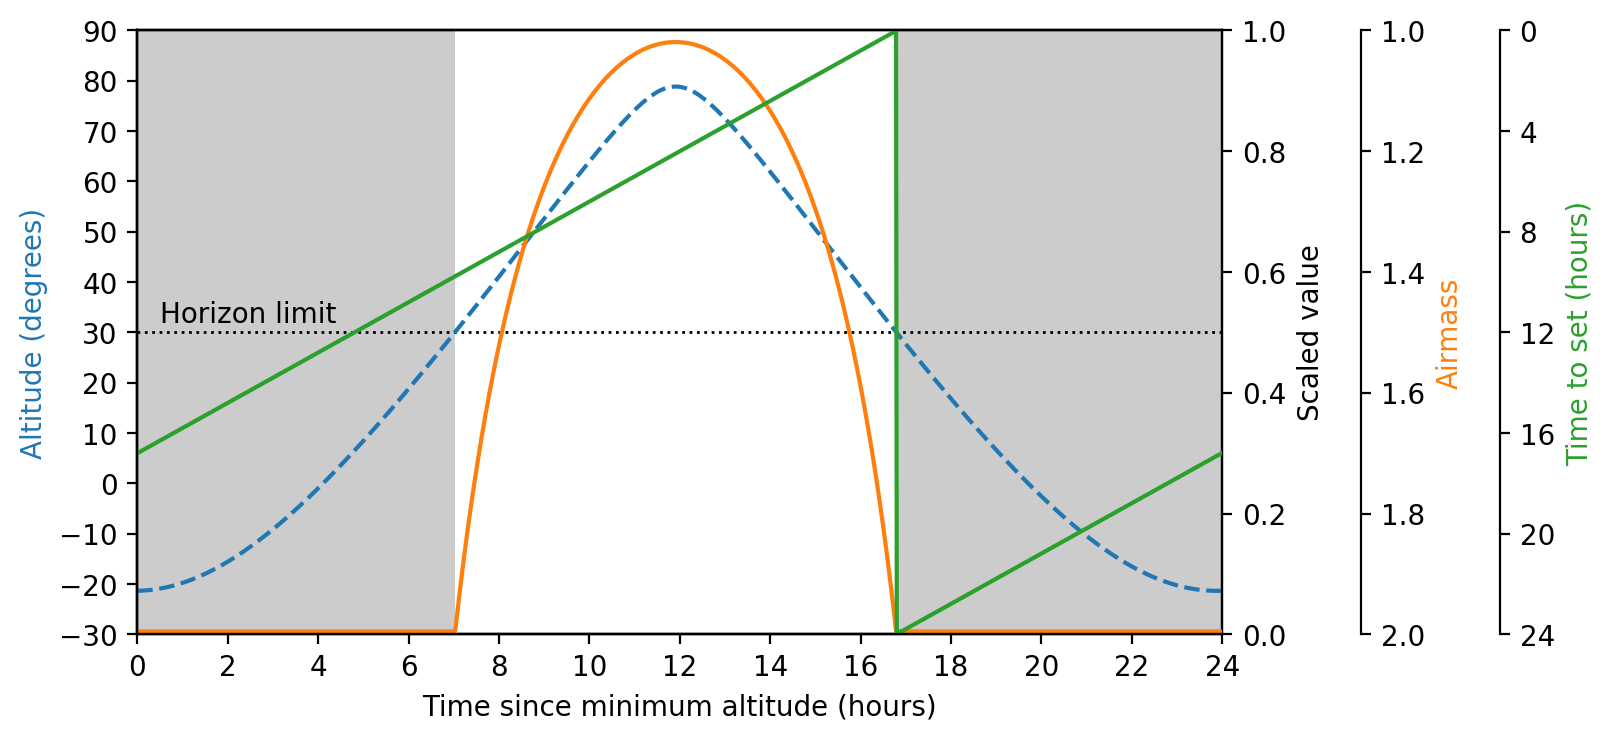
\includegraphics[width=\linewidth]{images/airmass-tts.png}
    \end{center}
    \caption[Defining airmass and time-to-set for a given target]{
        Defining airmass and time-to-set for a particular, arbitrary target. The altitude of the target is shown in \textcolor{Blue}{blue} over the course of one day and the corresponding airmass in \textcolor{BurntOrange}{orange}. The time-to-set is shown in \textcolor{Green}{green}, decreasing to 0 at the time the target passes below the \SI{30}{\degree} horizon (shown in red) and then resetting to the maximum. The grey regions are the times when the target is below the horizon.
    }\label{fig:airmass_tts}
\end{figure}

\begin{figure}[p]
    \begin{center}
        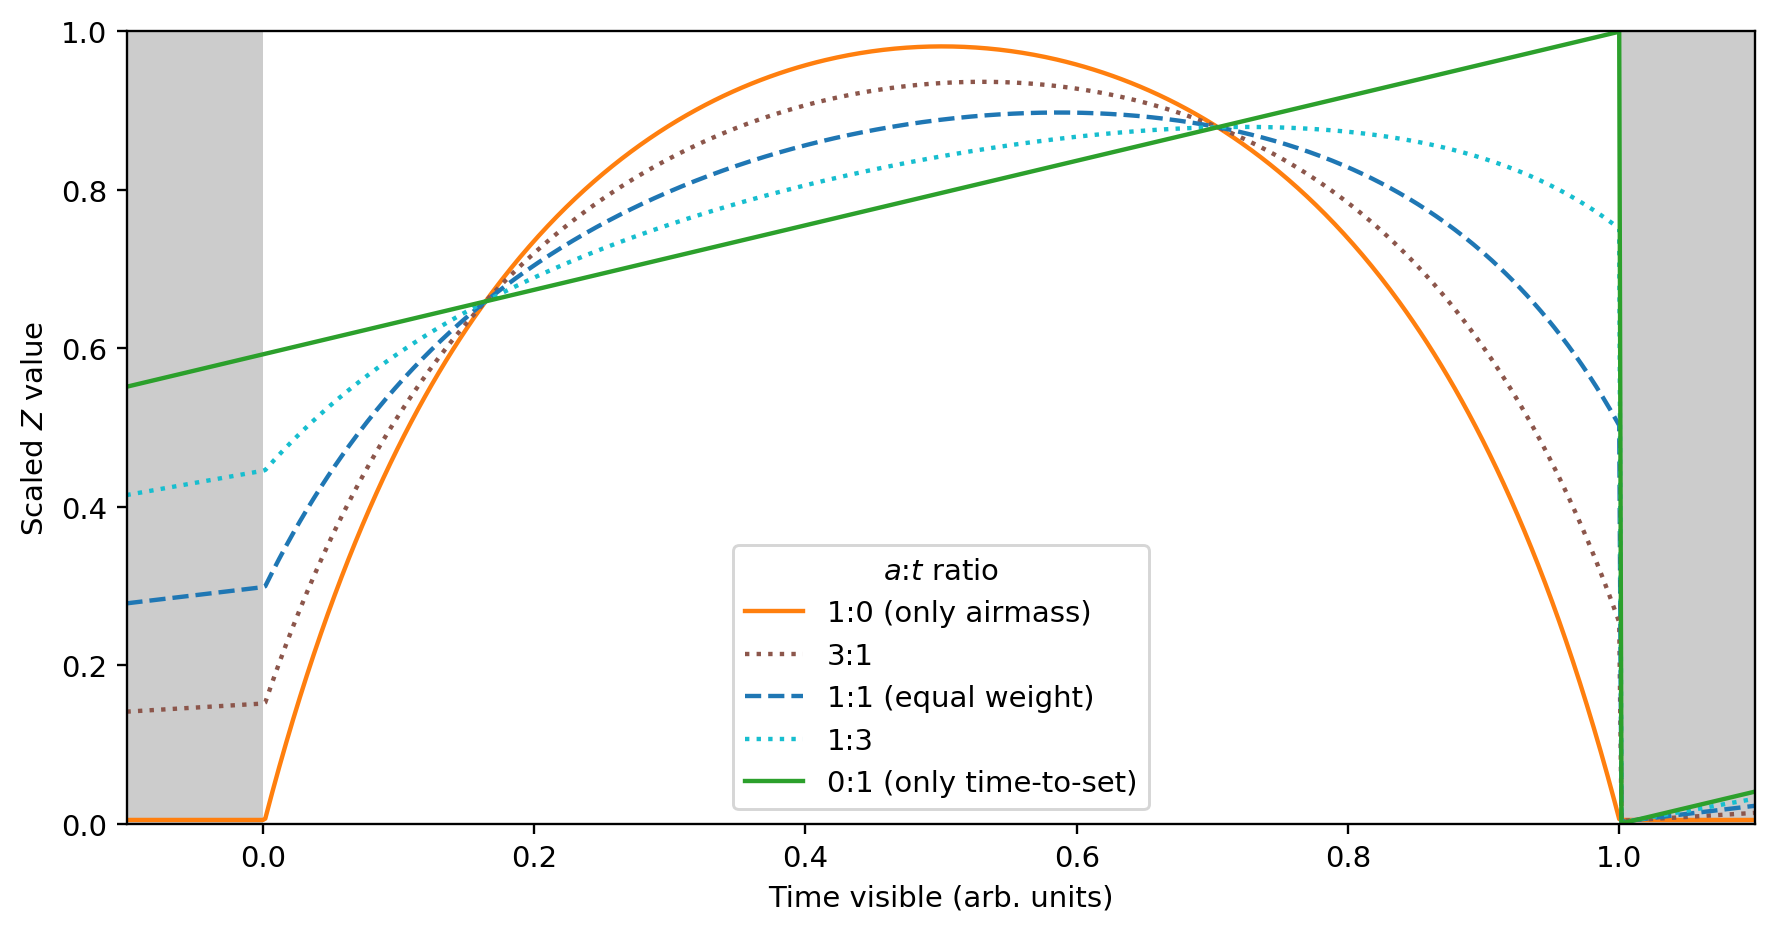
\includegraphics[width=\linewidth]{images/at_ratio.png}
    \end{center}
    \caption[Combining airmass and time-to-set with different ratios]{
        Combining airmass and time-to-set with different ratios. Increasing the relative weighting towards time-to-set shifts the peak of the overall distribution to the right.
    }\label{fig:at_ratio}
\end{figure}

\clearpage

% ---------
\subsubsection{The PAT ratio}

The previous sections detail three different parameters to be considered as part of the scheduler tiebreak parameter: the contained tile probability ($P$), the airmass ($X$) and time-to-set ($T$). Combining these parameters will provide a single, weighted value for each tile at the scheduler check time as

\begin{equation}
    \text{Tiebreak parameter} = \frac{p}{p+a+t} P + \frac{a}{p+a+t} X + \frac{t}{p+a+t} T.
    \label{eq:pat}
\end{equation}

where $p$, $a$ and $t$ are the weightings for the probability, airmass and time-to-set respectively. Together these are called the PAT ratio, and are usually written in the form $p$:$a$:$t$. So a PAT ratio of 1:1:1 means all three are weighted equally, where as 2:1:1 means probability is weighted twice as much as airmass or time-to-set.

\end{colsection}

% ~~~~~~~~~~~~~~~~~~~~

\end{colsection}

% ########################################

\newpage
\section{Scheduler simulations}
\label{sec:scheduler_sims}
\begin{colsection}

% ~~~~~~~~~~~~~~~~~~~~

\begin{colsection}

The first simulations of the \gls{gtecs} system were carried out in 2016 when the target scheduling code was being written. The scheduler needs a way to distinguish equally-ranked pointings, as described below, and the choice of weightings for this `tiebreaker' needed to be decided on. Therefore a series of simulations were carried out in order to find which weightings gave the best performance when observing gravitational wave skymaps.

\end{colsection}

% ~~~~~~~~~~~~~~~~~~~~

\subsection{Simulating GOTO}
\label{sec:goto_sims}
\begin{colsection}

The GOTO Telescope Control System (G-TeCS) described previously contains all the code used to operate the GOTO telescope. The intention of these simulations is to model the response of the real telescope using the real code as much as possible. The G-TeCS module contains test systems down to the level of the individual daemons and hardware units, meaning it is possible to simulate, for example, the camera daemon taking exposures using fake hardware code that waits in real time until the exposure time is completed (plus some readout time) and then creates a blank FITS image file with all the expected header information. On top of this the real pilot can run without knowing these daemons are fake, the real sentinel daemon can add real or simulated events into a copy of the observation database for the real scheduler to chose between. In this way the entire control system can be run without any of the real hardware.

The fully-featured test code described above is not ideal for the simulations carried out in this chapter: ideally the simulations would run faster than real time, and it is not necessary to simulate the full system down to fake images being written out. In these simulations everything below the pilot is abstracted away, and the pilot itself is replaced by a new specialised script simply called the fake pilot. This contains a class \code{FakePilot} that mirrors the real \code{Pilot} in several ways, such as the scheduler checks and deciding what to observe. There are however several important simplifications:

\begin{itemize}
    \item Firstly the pilot does not call the scheduler daemon in order to find what pointing to observe, but instead just imports and runs the scheduling functions itself. This was the original way the pilot ran before the scheduler was split into a separate daemon, as described in \aref{sec:scheduler}.
    \item Secondly the pilot does not bother with the full conditions checks and the conditions daemon. The \code{check\_conditions} routine still exists in order to ``close the dome'' (stop observations) when the Sun has risen, but is just a single function check. There was code written to simulate weather closing the dome with random Gaussian processes, however this was not used in any of the simulations as it would just distract from their purpose.
    \item The night marshal and any observing tasks other than actually observing the scheduler target (e.g.\ autofocusing) have been removed. Observations start immediately after sunset and continue to sunrise, and then when the dome is closed the pilot loop continues until the simulation has completed. Related to this the fake pilot can be run for multiple nights, instead of exiting and needing to be restarted.
    \item While the real pilot works using loops that sleep until a given time has passed, the fake pilot contains an internal time which is increased for each `step' in the simulation. At each step the script checks the scheduler using the normal commands. One important factor in speeding the simulations up is to increase this step size, up to the point that each observation takes a single step. This means that at each step the pilot will observe a new target, and increase the internal simulation time by the appropriate amount (for example if the target pointing asks for 3 60s \textit{L} exposures the simulations would increase by 3 minutes, plus extra time for readout and slewing to the target before the exposures start).
\end{itemize}

The fake pilot allows the response of the telescope to be simulated, based on the input pointings in the observation database. The database structure remains identical to the real thing, and pointings are defined either using the default all-sky survey settings (for \aref{sec:survey_sims}) or the GOTO-alert functions described in \aref{sec:gotoalert} for gravitational wave skymaps.

The first set of simulations were carried out early on in the development of G-TeCS, when the GOTO telescope was still under construction in La Palma. These were used to find values for the scheduler tiebreaker algorithm to best optimise gravitational wave skymap coverage without compromising too much on data quality. These simulations are described in \aref{sec:scheduler_sims}.

As described in \aref{sec:goto_expansion}, the ultimate aim of the \gls{goto} project is to have multiple nodes around the world. Specifically, the plan calls for two full GOTO-8 systems on La Palma and another two at a second site in Australia (the exact site is not yet determined, but it will most likely be either Siding Spring in New South Wales or Mt Kent in Queensland). In order to better quantify the benefit multiple telescopes and sites will provide, a series of simulations were carried out to model the combined system's response to gravitational wave alerts (in \aref{sec:gw_sims}) and the coverage and cadence of the all-sky survey (\aref{sec:survey_sims}).

\end{colsection}

% ~~~~~~~~~~~~~~~~~~~~

\subsection{Simulation results}
\label{sec:scheduler_sim_results}
\begin{colsection}

A series of simulations were carried out in order to find optimal values for the PAT ratio, and see how the telescope response changes depending on the ratio used. The fake pilot and scheduler code described in the previous section was run with a selection of skymaps from the LIGO First Two Years project \citep{First2Years}. The PAT ratio was set within the scheduler code, and the skymaps were then added to the observation database and the fake pilot ran through one night of simulated observations for each.

Two primary metrics were used to judge the effectiveness of the simulations. The first was the fraction of the skymap probability covered during the simulated night of observations, the total contained probability within all the tiles that were observed. The second was the mean airmass of each tile when observed. The average of these two values across all the skymaps for the different PAT ratios simulated are plotted in \aref{fig:scheduler_sim_results}.

\begin{figure}[t]
    \begin{center}
        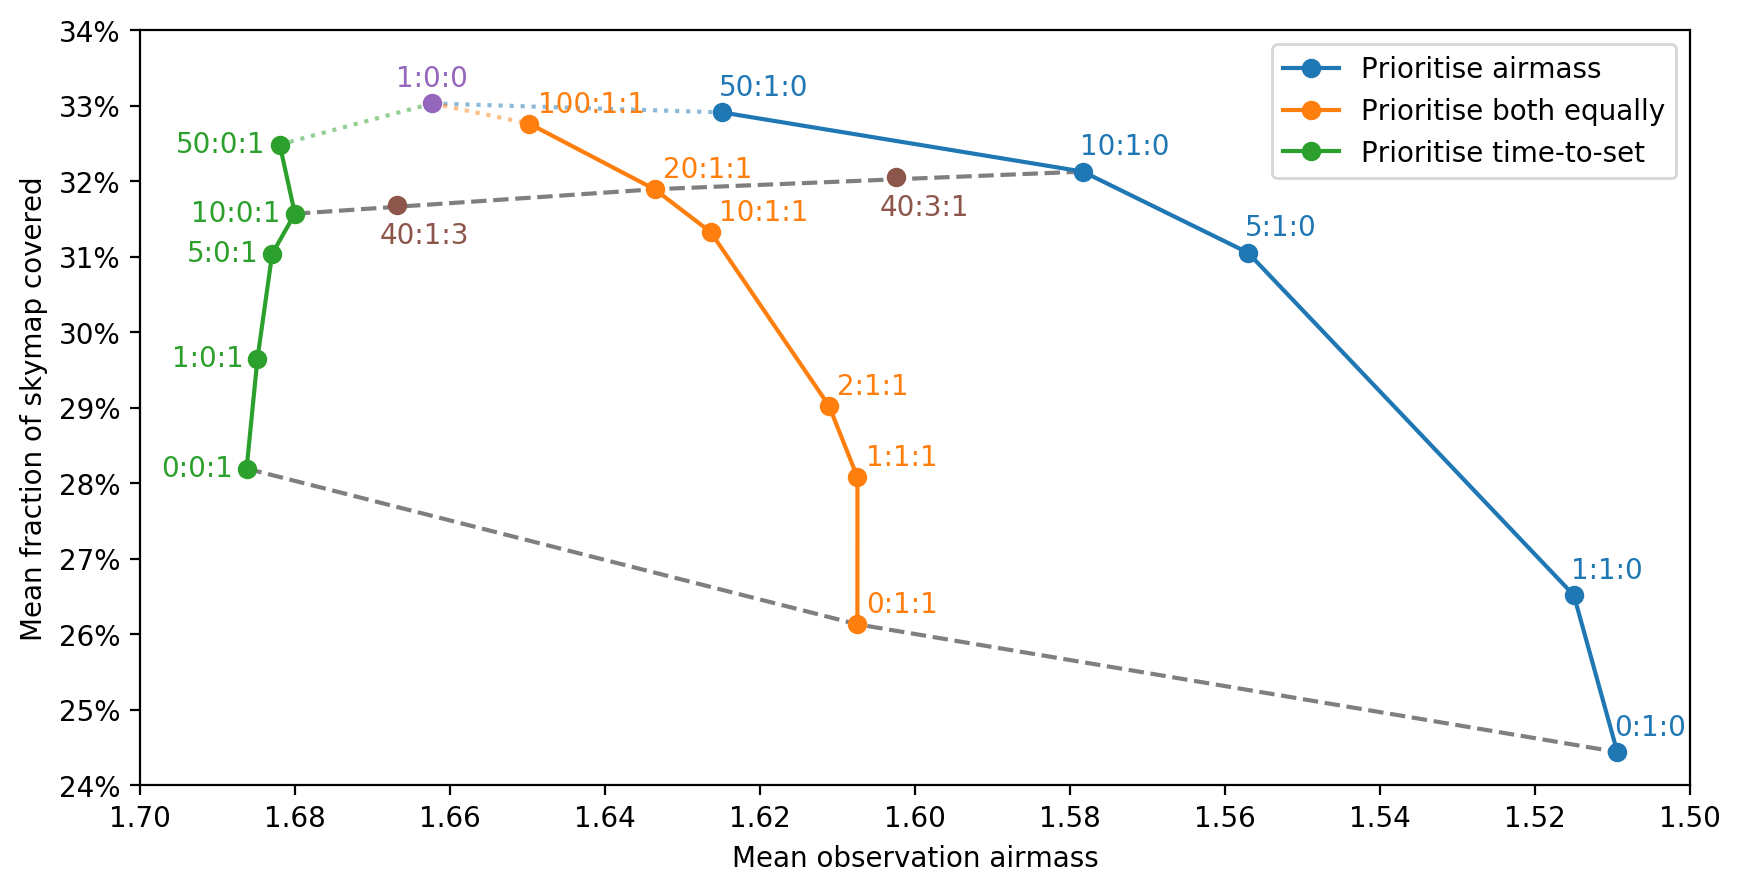
\includegraphics[width=\linewidth]{images/scheduler_sim.png}
    \end{center}
    \caption[Airmass vs fraction of skymap covered for different scheduler weightings]{
        Mean observation airmass vs fraction of the event skymap covered for different scheduler weightings. The full coloured lines join simulations with common airmass:time-to-set ratios, while the dashed lines show some simulations with the same probability weighting relative to the other two parameters. The region formed by the 1:0:0, 0:1:0 and 0:0:1 points contains all possible ratios. The optimal target is low airmass and high fraction covered, corresponding to the top-right of these axes.
    }\label{fig:scheduler_sim_results}
\end{figure}

\end{colsection}

% ~~~~~~~~~~~~~~~~~~~~

\subsection{Analysis of simulation results}
\label{sec:scheduler_sim_analysis}
\begin{colsection}

\aref{fig:scheduler_sim_results} shows several clear trends that emerge from modifying the PAT ratios. Increasing the relative weighting of probability compared to the other two parameters (from 0:X:X, 1:X:X, 5:X:X up to 1:0:0 which is effectively $\infty$:X:X) increases the mean probability covered by up to a third, from 24\% to 33\%. This however typically comes at a cost to the mean airmass of the observations.

Changing the relative ratios of airmass to time-to-set (from Y:1:0 to Y:0:1) shows an unexpected result. It is true the observed airmasses would be lower as less weight is put on the airmass parameter, however it was intended that introducing the time-to-set parameter would compensate by catching more setting tiles that would be missed purely looking around the zenith. This is the result if probability is not included as a factor, as seen by the 0:0:1--1:0:0 line at the bottom of \aref{fig:scheduler_sim_results}. When only airmass is considered (in the 0:1:0 case) the results produce the best average airmass per observation but the worse skymap coverage. On the other hand only considering time-to-set (0:0:1) results in worse airmasses but better coverage. But having the explicit probability parameter counteracts this trend. Looking at the 10:0:1--10:1:0 line changing the airmass to time-to-set ratio only reduces the mean airmass with no corresponding gain in probability covered. In the case where the airmass parameter is ignored (the green time-to-set line on the left of \aref{fig:scheduler_sim_results}) the inclusion of the time-to-set value is just actively suppressing the amount of probability observed while making almost no difference to the mean airmass.

Based on these results, it is clear that the optimal solution is to ignore time-to-set and chose a tiebreaker PAT ratio of around 5:1:0 to 10:1:0, to get the best airmass while limiting the coverage lost. The final scheduler has been operating with a ratio of 10:1:0, as compared to 5:1:0 this gives a gain in mean airmass only 0.02 airmass while increasing the skymap coverage by 1\%. This is only restricting the options to the ratios simulated however, and further simulations would be able to explore the parameter space further.

The results plotted in \aref{fig:scheduler_sim_results} show remarkably smooth trends. The three coloured lines with fixed airmass:time-to-set ratio all curve and trend towards the 1:0:0 point, aside from the slightly outlying 50:0:1 point. The points with a fixed probability weight compared to the other two also seem to form straight lines, as shown by the 10:0:1 to 10:1:0 line. As only the relative values of the ratios matter the 20:1:1 point could be considered to be 10:\sfrac{1}{2}:\sfrac{1}{2}, likewise 40:1:3 and 40:3:1 are 10:\sfrac{1}{4}:\sfrac{3}{4} and 10:\sfrac{3}{4}:\sfrac{1}{4}, from this it is clear that any ratio of airmass to time-to-set will fall on this line if together they add to one-tenth of the probability weighting. However the results shown in \aref{fig:scheduler_sim_results} should be taken with caution. As each point is based on the means over multiply skymaps there is a wide range of variation, and in fact were error bars be included they would have spread off the page in both axes.

The conclusions on the PAT ratio made above are not unreasonable if all that is needed is a one-size-fits-all set of values that are hard-coded into the scheduler, as the current system does use. However when these simulations are revisited it would be a good idea to look more in detail at other trends that might be hidden in the averages. For example if one ratio might be better suited for large skymaps vs smaller ones, or in cases where the whole skymap is visible at once compared to it slowly rising up during the night. These simulations also only considered visibility from La Palma and observed for just the first night, rather than the full 24 hours as used by simulations described later.

These simulations were carried out as the scheduler was still being designed, and long before any of the sentinel or GOTO-alert functions described in \aref{sec:gotoalert} were written. The simulations used the original GOTO-tile code written by Evert Rol to split the skymaps up into the grid, and the individual pointings then had to be added separately into the database. The process in general was a lot slower and required manual intervention to reset the database and ratio values, which is why it took longer to run and fewer simulations were run compared to those described later in this chapter. This was also before GOTO construction began on La Palma, and so properties like the field of view and horizon had to be assumed. Repeating these simulations with the newer code is needed to see if the conclusion that 10:1:0 is still the best case, and at the same time examine the possibility of modifying the ratio based on properties such as the extent of the skymap and time of the event.

Finally, other possible values could be considered for inclusion in the ``PAT'' ratio. One suggestion is to modify time-to-set into time-visible, by including not only the time when the target sets below the horizon but also the time that the Sun rises. The existing time-to-set ratio prioritises observing targets later in the night when they are about to set, where as airmass prioritises tiles near the zenith. Neither however considers the time remaining in the night, and while this is obviously the same for every target it would be better for the time-to-set distribution to peak before sunset instead of after to best prioritise observations in the limited time available.

\end{colsection}

% ~~~~~~~~~~~~~~~~~~~~

\end{colsection}

% ########################################
